\documentclass[12pt]{article}

\usepackage{graphicx}
\usepackage{longtable}
\usepackage{hyperref}
\usepackage{textcomp}
\usepackage{float}
\usepackage{vhistory}

\graphicspath{ {images/} }

\begin{document}

\begin{titlepage}
	\centering
	{\scshape\LARGE McMaster University \par}
	\vspace{1.5cm}
	{\huge\bfseries User Manual \par}
	{\scshape\Large Revision 1 \par}

	\vspace{1cm}
	{\scshape\Large Capstone Team 14\par}
	{\Large\itshape Ananthan Kanagasabai, Andrei Ciontea, Curran Tam, Joseph Nguyen, Victor Siu \par}
	\vspace{3cm}
	\vfill
	supervised by\par
	Dr.Sarah Khan, Wenbo He

	\vfill
	{\large \today\par}
\end{titlepage}

\newpage

\tableofcontents
\listoffigures

\newpage

\section*{Revision History}
\begin{tabular}{|c|c|}
\hline
\textbf{Date}  & \textbf{Comments} \\ \hline
March 6, 2017 & Revision 0 of User Manual created \\ 
\hline
April 9, 2017 & Correction and Final Revision\\
\hline
\end{tabular}

\newpage


\section{Introduction}
The HIV Regimen Generator is a website that be used by doctors to create a combination of ARV medications. The generated output is analyzed by the doctor and the best available option is given to a patient with HIV. The website consist of a form that allow the client (the doctor in this case) to enter a series of inputs pertaining to the patient's medical history and requirements. The form display input options related to the patient and the type of medication they can receive. After the doctor has selected or entered the required inputs, they are redirected to a page that displays their inputted form data, along with the medication combinations that our algorithm would be generate. The medication being also displayed have a description and other information associated with its use and side effects.

\section{Copyright}
HIV Regimen Generator is owned and managed by Team 14 of CS4ZP6. The team is a part of McMaster University. The collaborators on the project are: Ananthan Kanagasabai, Andrei Ciontea, Curran Tam, Joseph Nguyen and Victor Siu. This project is hosted on GitHub. The license of Common Development and Distribution License (CDDL-1.0) is used for fair use.

\section{About this Manual}
This manual report how the website be operated and inform first time users how to navigate and use the HIV Regimen Generator to its full potential. The manual describe the webpages associated with it first, as well as their purpose and how to navigate between them. Then the manual describe existing errors/issues and the steps required to correct them. Finally, the section at the end of this document answer common questions associated with the project.

\newpage
\section{Naming Conventions and Terminology}
\begin{itemize}
	\item ARV: Antiretroviral drug
	\begin{itemize}
		\item Medication that is given to patients who are HIV positive
	\end{itemize}
	
	\item BSA: Body Surface Area
	\begin{itemize}
		\item Value that is calculated by using the weight and height of a person to predict dosage requirements
	\end{itemize}

	\item Tanner Stage
	\begin{itemize}
		\item A scale of physical development in children, adolescents and adults; this is used to determine the amount of dosage to give the patient
	\end{itemize}
\end{itemize}

\section{Browser Requirement}
The HIV Regimen Generator is compatible and has been tested with the following web browsers:
\begin{itemize}
	\item Google Chrome ver. 55.0.2883
	\item Mozilla Firefox ver. 52.0.2
	\item Internet Explorer 11
\end{itemize}

\section{Tasks}
\subsection{Start}

The Start page (Figure 1) is the landing page of the website. On this page, the website logo is displayed. 

\begin{itemize}
	\item A “Start Here” button is also available which redirect the user to the Form page where patient information be entered.
	\item  The navigation menu at the top of the page features a Home option, that takes the user back to the landing page.
	\item There is also an About option on the navigation menu that serves as an information/tutorial page.
\end{itemize} 

\begin{figure}[H]
  \centering
  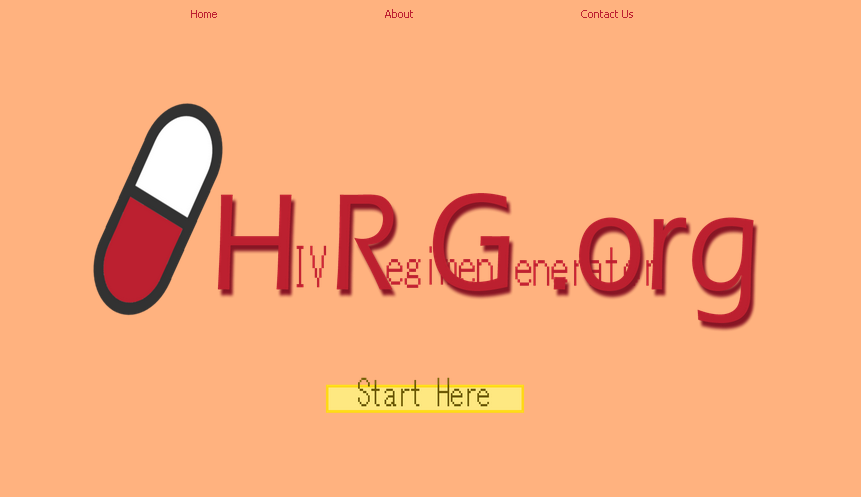
\includegraphics[width=\linewidth]{landing.png}
 \caption{Screen image of the Landing/Main page}
  \label{fig:landing}
\end{figure}

\subsection{Form}
This page (Figure 2) is a form that asks for the medical information of the patient. 
\begin{itemize}
	\item It first asks for any preliminary information such as: age, height, and weight.
	\item Next is the “Calculate BSA” button, which calculates the body surface area of a person based on the inputted height and weight.
	\item  The Tanner stage is used to measure the physical development in an adolescent.
    \item HLA refers to the human leukocyte antigen, which is a gene complex that determine whether or not to give the abacavir medications. 
    \item  Next is a checklist of the medical issues that are present in the patient, as well as any applicable resistances.
    \item The form also asks for allergies which could potentially conflict with prescribed medication and thus the system need to reweigh its suggested options.
\end{itemize}
  Depending on the age of a child, some forms of applying medication cannot be used, so the form provides the user with an option of selecting the type. After Submitting this form, it would be take you to the combo page.

\begin{figure}[H]
  \centering
  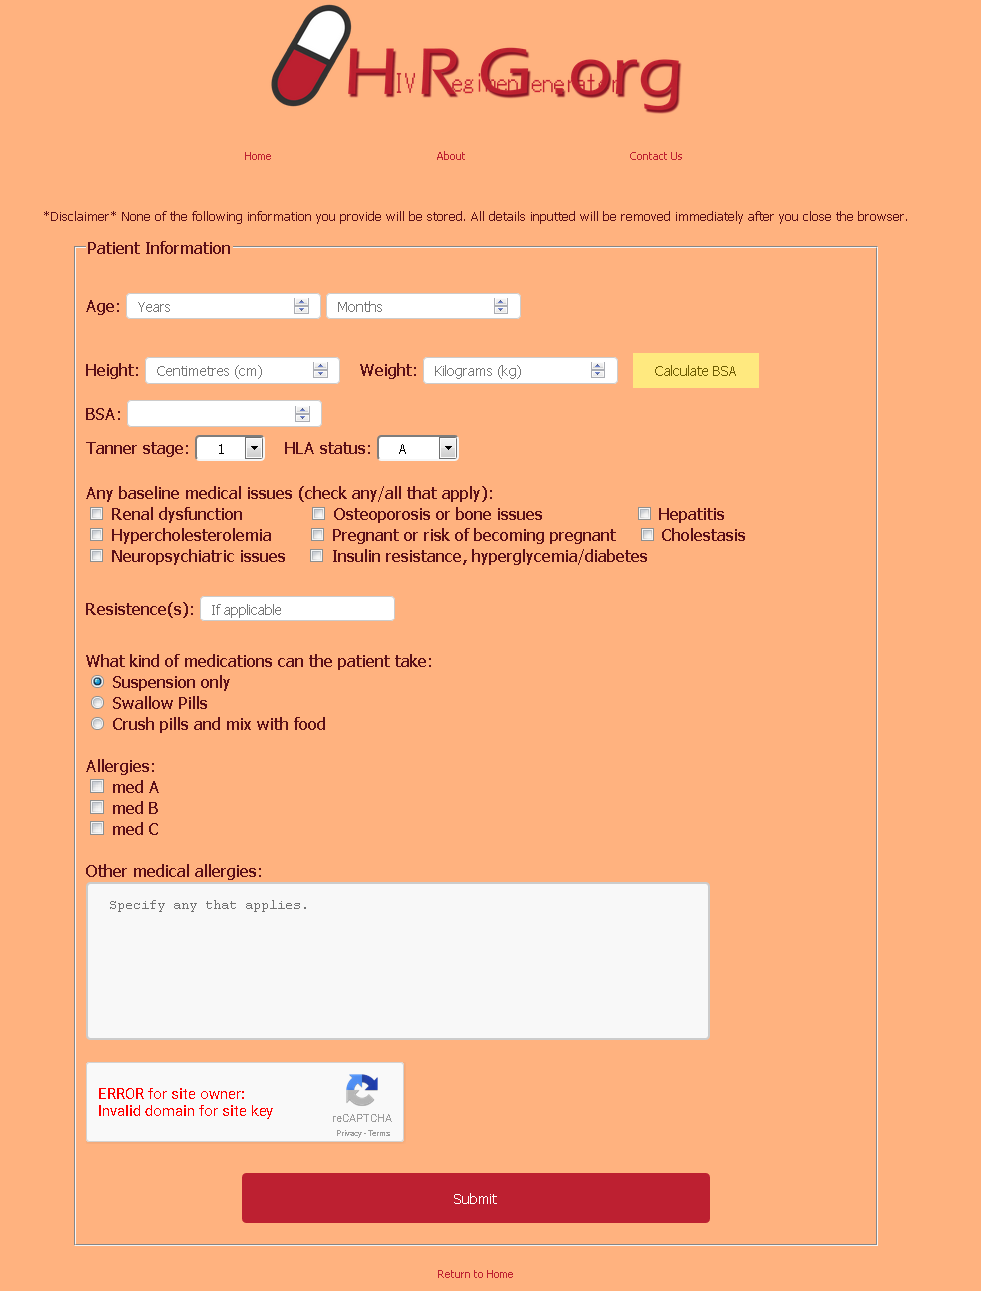
\includegraphics[width=\linewidth]{form1.png}
  \caption{Screen image of Patient Information page; the form}
  \label{fig:form1}
\end{figure}

\subsection{Combo}
The Combo page (Figure 3) is displayed after the client has filled out the required information on the Form page. 
\begin{itemize}
	\item This page display a few possible combinations of medications that may be used by the patient.
	\item  The client then selects one of the combinations by clicking on a button beside the desired combination.
	\item When the client has made their final decision on what combination they want to work with, they can click on the Submit button to be taken to the Results page.
\end{itemize}

\begin{figure}[H]
  \centering
  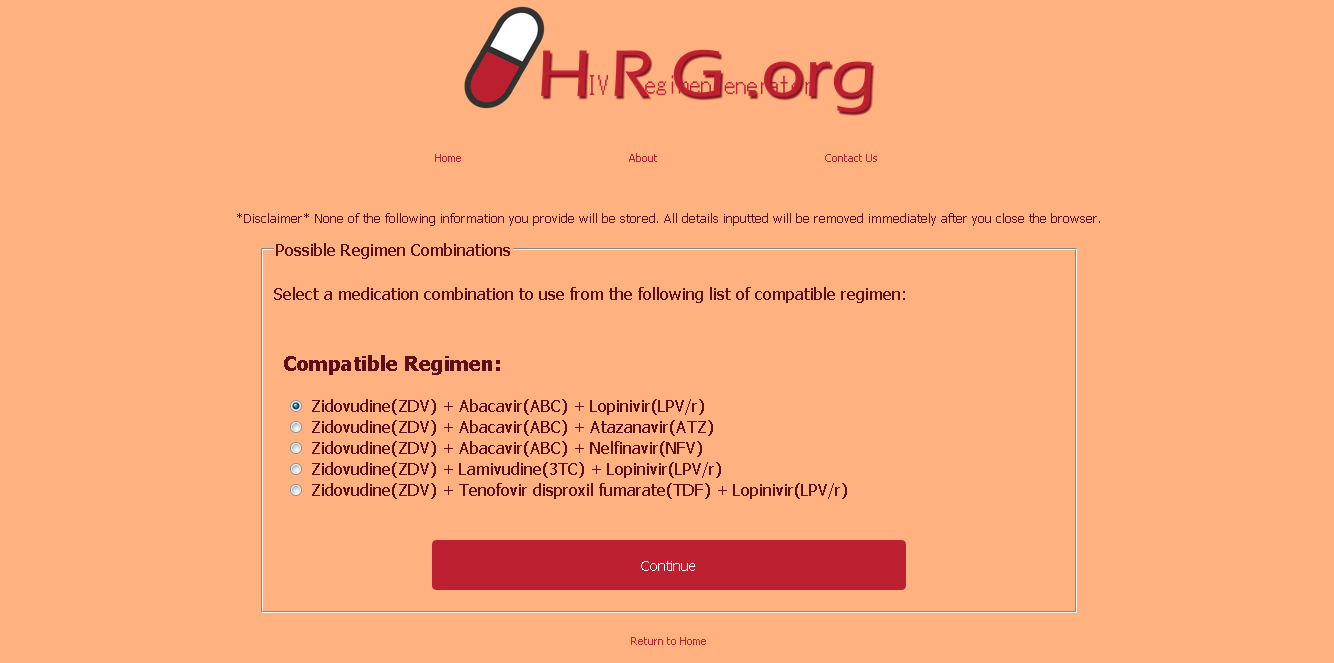
\includegraphics[width=\linewidth]{combo.png}
  \caption{Screen image of Combination Selections page}
  \label{fig:combo}
\end{figure}

\subsection{Results}
The Results page (Figure 4) is a final information page which displays the patient information at the top, containing all the details that were written on the form. Below the patient information are the details of the regimen that was selected on the combo page.\\\\ This provides a more detailed description of each medication, as well as their: suggested dosage, potential side effects, and a link to a reference should the user have any further inquiries.

\begin{figure}[H]
  \centering
  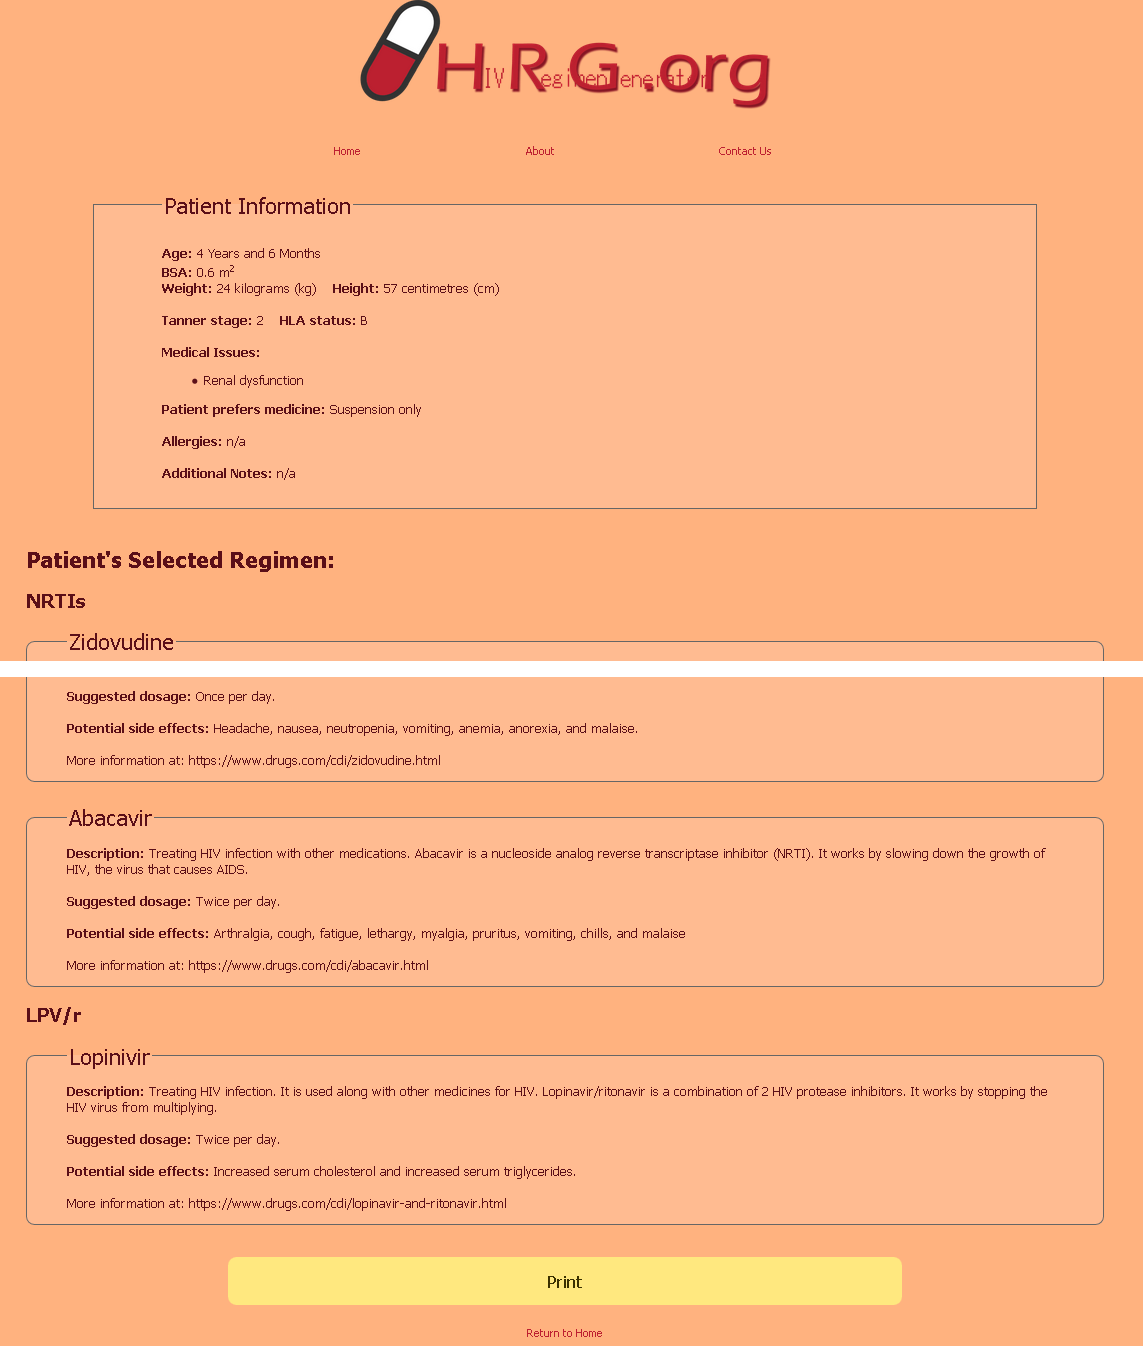
\includegraphics[width=\linewidth]{results1.png}
  \caption{Screen image of Medical Results page}
  \label{fig:results1}
\end{figure}

\subsection{About}
The About page gives detailed information about the purpose of our website. The purpose  is to provide a regimen to any HIV positive patients. This page is also contain information about the team, as well as provide this user manual and a tutorial on how to operate the website.

\section{Troubleshooting}
\subsection{Overview}
The team has taken the necessary precautions so that no errors from the website are negatively affect a client's personal operating system. The website is tested before it is uploaded the Internet. This part of the document address any problems that arise as a result of being on this website.

\subsection{Internet Connection}
The client must use a machine with a working Internet connection to access this website. Otherwise, no web page is displayed.

\subsection{Slow Loading}
Any pages that are loading slowly are a result of an overload to the server or a slow Internet connection.

\section{Frequently Asked Questions}
Q: Can we get more details of the drug that we can use?\\
A: Yes. After getting results, there is a link to go to \url{https://www.drugs.com/} in the Patient’s Selected Regimen of result page. You can click the link to see any information about the drugs.\\\\
Q: Is this site accurate?\\
A: Yes. This website has been tested by both the developers of the algorithm and the doctor that we have been working alongside.\\\\
Q: How updated is the medical database being used?\\
A: The medical database is up to date as of February 28, 2017. Further improvement of this algorithm could allow us to extract information from an existing website to detect new medications and discoveries.\\\\
Q: How does a patient's sensitive information be protected?\\
A: Information about the patient does not recorded. This algorithm simply receives information and outputs medications without any information that identify or keep a record of any specific patient.\\\\
Q: Where can I find your web application?\\
A: The application is not currently hosted on any web services at the moment. The program can be accessed locally with a local APACHE host and mysql database server using XAMPP.

\end{document}